\chapter{Wprowadzenie}

Naszym celem było ukazanie w jaki sposób można zaimplementować web-scraping w aplikacji internetowej. Chcieliśmy sprawić, aby web-scraping był tylko jedną składową z komponentów, które zaimplementowaliśmy w programie.

Pomysł na naszą aplikację narodził się podczas odbywanych przez nas licznych wizyt w galeriach handlowych, gdzie zauważyliśmy jak dużo czasu, wysiłku i pieniędzy ludzie poświęcająm aby do posiadanej odzieży dopasować nowe elementy garderoby.

Na taki stan rzeczy składa się kilka czynników. Pierwszym z nich jest dostępność produktów. Wybór konsumenta ograniczony jest przez wyposażenie sklepów na terenie galerii. Ponadto, konsument ma tendencję do kupienia produktu, który w jego mniemaniu jest nabliższy temu, czego oczekiwał, lecz często nie dokładnie taki. To pokazuje nam kolejny problem - konsument nie pożytkuje swoich pieniędzy najlepiej, jak to możliwe. Nie sposób jest porównać wszystkich przedmiotów z puli potencjalnych dopasowań, ponieważ są one rozproszone po różnych sklepach, często galeriach, a nawet miastach. 

Trzecim czynnikiem jest czas poświęcony na wybieraniu potencjalnych dopasowań, ponieważ koniecznym jest fizycznie udać się do sklepów.

Jednym z rozwiązań problemu braku czasu jest zatrudnienie stylisty, który podpowie, które dopasowanie jest najlepsze, lecz jest to kosztowna usługa, na którą nie każdy może sobie pozwolić.

Odpowiedzią na te problemy jest nasza aplikacja. Po wprowadzeniu w pasku wyszukiwarki produktu, prezentowana jest użytkownikowi lista najlepiej skomponowanych do niego artykułów wraz z linkiem do sklepu, zdjęciem oraz ceną.
Wystąpienie na liście propozycji dopasowania podyktowane jest jego popularnością oraz częstotliwością doboru wśród innych użytkowników systemu.
Pozwala to na oszczędzenie czasu poprzez możliwość porównania bez wychodzenia z domu.
Aplikacja przyczynia się również do oszczędności pieniędzy, ponieważ niejako eliminuje potrzebę zatrudniania stylisty.

Produkt działa z wykorzystaniem web-scrapingu opartego na pythonowym frameworku Scrapy.
Poniższy diagram przedstawia po krótce proces działania wspomnianego modułu.

\begin{figure}[h]
    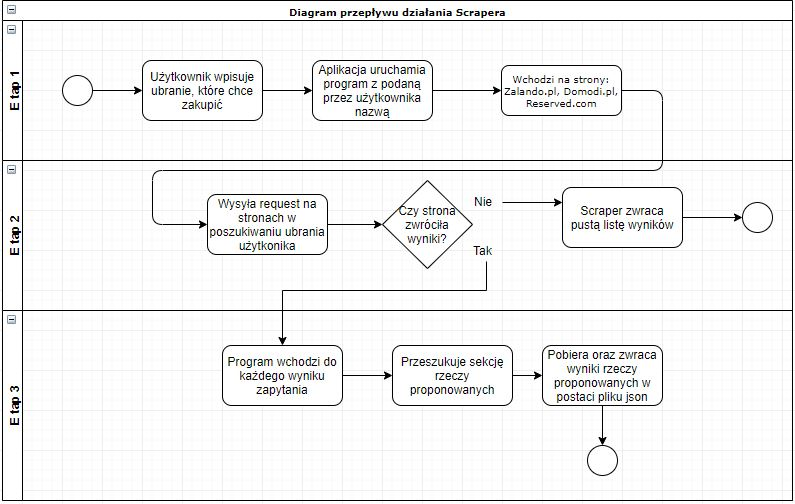
\includegraphics[width=1.1\textwidth]{zdjecia/diagram}
    \caption{Diagram działania scrapera. Wykonanie własne}
\end{figure}

Wyszukiwania są cachowane na serwerze pośredniczącym, co pozwala użytkownikowi na szybsze wyszukiwanie i płynniejsze korzystanie z aplikacji.
Zasoby statyczne takie jak zdjęcia pobierane są z serwera pośredniczącego, a nie z domeny docelowej.

Dodatkowym atutem korzystania z serwera pośredniczącego jest ukrycie prawdziwego adresu logicznego użytkownika, dzięki czemu utrudni to reklamodawcom prezentowanie mu reklam, co miałoby miejsce w przypadku bezpośrednich wizyt w poszczególnych domenach sklepów internetowych.sklepach

W projekcie wykorzystujemy load balancing, dzięki któremu ruch będzie rozpraszany na wszystkie węzły, a użytkownik nie odczuje spadku wydajnośći w przypadku wzmożonego ruchu.

\textbf{Słowa kluczowe:} web-scraping, dopasowanie ubrań, stylizacja modowa